
\chapter{Introduction}
    By the term \textit{Mobile robots} it is meant an ensemble of rigid bodies, equipped with a locomotion system. It is then understood that the ability of freely moving around their environment is the biggest difference between mobile and industrial robots, the latter being mostly bolted to the ground. \\
    Mobile robots are mainly distinguished by their locomotion systems:
    \begin{itemize}
        \item \textit{Wheeled Robots}: composed by one rigid body, the \textit{chassis}, to which wheels are attached (and trailers if needed).
        \item \textit{Legged Robots}: multiple rigid bodies, some of which mimic legs. The robot has multiple extremities (\textit{feet}) in periodic contact with the ground to achieve motion.
        \item \textit{Flying Robots}: composed by a rigid body, the \textit{frame}, to which either rotors or fixed wings are attached. Propellers represent the locomotion system.
        \item \textit{Underwater Robots}: very similar to flying robots, but with the additional care due to the environment in which they work.
    \end{itemize}
    Building mobile robots comes with some challenges, such as:
    \begin{itemize}
        \item \textit{Localization} in their (dynamic or static) environment; mobile robots can make use of encoders and GPS, but these either have many unmodelled dynamics or flat-out don't work in some environments and situations. Another complication is computational: Direct Kinematics is expressed by (often constrained) sets of differential equations. 
        \item State-Estimation or \textit{Odometry} is also very complex and has the goal of estimating the robot's position from either on-board or off-board sensors; often robots perform \textit{Simultaneous Localization And Mapping} (SLAM) online during execution of their tasks, making Odometry a very computationally heavy task.
        \item \textit{Motion Planning} is the job of computing a path and time law (a \textit{trajectory}) compatible with the environment. This is often done in real-time for mobile robots, making it again very difficult for the designer.
        \item \textit{Motion Control} is the task of determining the robot's inputs to follow the planned path. This is difficult because, opposite to industrial robotics, there are plenty unmodelled dynamic effect taking action on a mobile robots, some of which could not even be envisioned before deploying the robot itself.
        \item Last but not least, the control \textit{Architecture} has to be chosen. There are mainly four approaches:
        \begin{itemize}
            \item \textit{Reactive Architecture}: "don't think, act".
            \item \textit{Hybrid Architecture}: Think and Act simultaneously.
            \item \textit{Behavioural Architecture}: Think about the action modality.
            \item \textit{Deliberative Architecture}: Think, then act. This is the one adopted in this course, based on Propioceptive and Exteroceptive sensors and perception.
        \end{itemize}
    \end{itemize}
    \section{Configuration Space and Degrees of Freedom}
    As previously stated, a mobile robot is free to move in its environment, which immediately begs the question of how to describe such a system.
     The robot’s \textbf{configuration} is the specification of the positions of all points of the robots, which will be assumed as the interconnection of fully rigid links by means of joints. This simplification greatly reduces the number of parameters needed to describe the robot's full configuration; then, the minimum number of real-valued coordinates needed to represent the configuration is called \textit{Degrees Of Freedom} of the system. By merging the two definitions, the \textit{Configuration Space} of a robot can be defined as:
    \begin{definition}
        \textbf{Configuration Space}: The $n$-dimensional space, where $n$ is the robot's number of DoFs, containing all the possible robot's configurations is called the \textit{Configuration Space} (C-space). The configuration of a robot is represented by a point in its C-space.
    \end{definition}
    An unconstrained rigid body immersed in three dimensional space has 6 DoFs (3 translational and 3 rotational), meanwhile in 2D space it has only 3 (2 translational and 1 rotational), as is known from physics. In general, a simple formula for computing the number of DoFs is:
    \begin{gather*}
        \text{DoFs}=(\text{Sum of degrees of freedom of the single bodies})+\\-(\text{number of independent constraints})
    \end{gather*}
    This formula can be easily applied on mechanical systems, such as robots, and takes the name of \textit{Gr\"{u}bler's Formula}:
    \begin{definition}
        \textbf{Gr\"{u}bler's Formula}: Consider a mechanism of $N$ links, counting also the ground. Let $J$ be the number of joints, $m$ the DoFs of a rigid body in the considered space, $f_i$ the DoFs provided by joint $i$ and $c_i$ the number of constraints provided by joint $i$, where $f_i+c_i=m$, for all $i$. Then, the number of DoFs of the robot is at least: 
        \begin{equation}\label{Grubler's formula}
            DoFs = m(N-1)-\sum_{i=1}^{J}c_i=m(N-1-J)+\sum_{i=1}^{J}f_i
        \end{equation}
        The equation is exact in the case of fully independent constraints, otherwise it is a \textbf{lower bound} for the number of DoFs of the mechanism.
    \end{definition}
    Different joints can give different DoFs based on their structure; in the following table, the most famous joints and their respective characteristic are summarized:
   \begin{figure}[htbp!]
    \centering
    \begin{minipage}{0.48\textwidth}
        \centering
        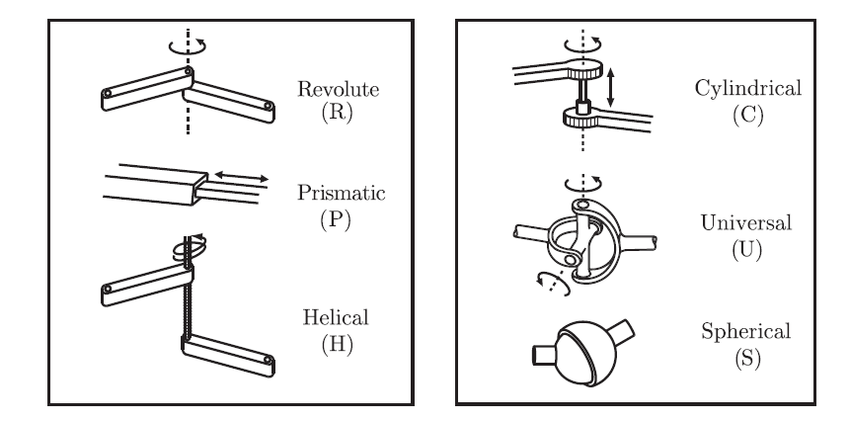
\includegraphics[width=\linewidth]{Images/typical_robot_joints.png}
    \end{minipage}\hfill
    \begin{minipage}{0.48\textwidth}
        \centering
        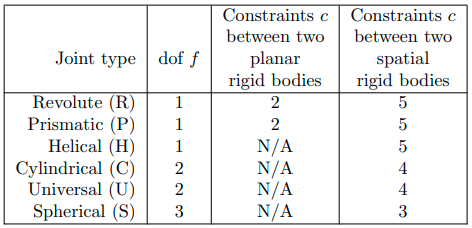
\includegraphics[width=\linewidth]{Images/image2.png}
    \end{minipage}
    \caption{Table of joints' characteristics.}
    \label{fig:joints_charas}
\end{figure}\\
\newpage
\subsection{Gr\"{u}ber's Formula examples}
    Let's see some examples of how to use Gr\"{u}bler's formula.
    \begin{itemize}
    \item Four bar Linkage \\
    
    
 \begin{figure}[htbp!]
                \begin{minipage}{0.4\textwidth}
                    We have 4 Links (considering the ground link) and 4 \textit{Revolute} Joints. We are considering the model in the plane, thus we have that 
\[
 N=4 (\text{four links}), J = 4 (\text{four joints}), m = 3 (\text{plane}),
 \]\[ f_i = 1 (\text{Revolute Joints in the plane})              
                    \]   
                    By applying Gruber's rule
                    \[DoFs=3(4-1-4)+4 = 1\]
                 
                \end{minipage}\hfill
                \begin{minipage}{0.5\textwidth}
                    \begin{tikzpicture}[>=stealth]

    % Definizione delle coordinate dei 4 giunti
    \coordinate (A) at (0,0);
    \coordinate (B) at (1.3, 3.4);
    \coordinate (C) at (4.7, 3.4);
    \coordinate (D) at (6,0);

    % Macro per disegnare i bracci di collegamento (Link - BLU)
    \newcommand{\drawlink}[2]{
        % Riempimento azzurro chiaro
        \fill[blue!20] ($(#1)!4mm!-90:(#2)$) -- ($(#2)!4mm!90:(#1)$) -- 
                       ($(#2)!4mm!-90:(#1)$) -- ($(#1)!4mm!90:(#2)$) -- cycle;
        % Bordi blu
        \draw[thick, blue] ($(#1)!4mm!-90:(#2)$) -- ($(#2)!4mm!90:(#1)$);
        \draw[thick, blue] ($(#1)!4mm!90:(#2)$) -- ($(#2)!4mm!-90:(#1)$);
    }

    % Macro per disegnare i supporti a terra (Telaio - NERO)
    \newcommand{\ground}[1]{
        \begin{scope}[shift={(#1)}]
            \draw[thick] (-0.6, -0.4) -- (0.6, -0.4);
            \foreach \i in {-0.5, -0.3, -0.1, 0.1, 0.3, 0.5} {
                \draw (\i, -0.4) -- (\i-0.15, -0.6);
            }
        \end{scope}
    }

    % 1. Disegno i tre bracci (collegamenti) - Colore BLU
    \drawlink{A}{B}
    \drawlink{B}{C}
    \drawlink{D}{C}

    % 2. Disegno i giunti (cerchi esterni e perni interni) - Colore ROSSO
    \foreach \p in {A,B,C,D} {
        % Cerchio esterno con riempimento rosso chiaro e bordo rosso
        \filldraw[thick, draw=red, fill=red!20] (\p) circle (4mm);
        % Perno interno con bordo rosso e riempimento bianco
        \filldraw[thick, draw=red, fill=white] (\p) circle (1.5mm);
    }

    % 3. Disegno i supporti a terra nei punti A e D
    \ground{A}
    \ground{D}

    % ==========================================
    % 4. ETICHETTE (LABELS) COLORATE
    % ==========================================
    
    \tikzset{etichetta/.style={font=\sffamily\small}}

    % Etichette per i giunti (Rosse)
    \node[etichetta, text=red, anchor=east]       at ($(A) + (-0.5, -0.1)$) {joint 1};
    \node[etichetta, text=red, anchor=south east] at ($(B) + (-0.4,  0.4)$) {joint 2};
    \node[etichetta, text=red, anchor=south west] at ($(C) + ( 0.4,  0.4)$) {joint 3};
    \node[etichetta, text=red, anchor=west]       at ($(D) + ( 0.5, -0.1)$) {joint 4};

    % Etichette per i bracci (Blu)
    \path (A) -- (B) node[midway, left=0.4cm, etichetta, text=blue] {link 1};
    \path (B) -- (C) node[midway, above=0.4cm, etichetta, text=blue] {link 2};
    \path (D) -- (C) node[midway, right=0.4cm, etichetta, text=blue] {link 3};
    
    % Etichetta per il telaio (Nera)
    \path (A) -- (D) node[midway, below=0.6cm, etichetta] {link 0 (frame)};

\end{tikzpicture}
                \end{minipage} 
            \end{figure} 
Now here it comes the most complex part: understanding the presence of dependent constraints. By reasoning about the model we can notice that by moving just one joint, the position of all the other joints is imposed, thus we showed that the number of DoFs is properly one.
\item Slider-Crank \\
   
 \begin{figure}[htbp!]
                \begin{minipage}{0.4\textwidth}
                    We have 4 Links (considering the ground link) and 4 \textit{Revolute} Joints. We are considering the model in the plane, thus we have that 
\[
 N=4 (\text{four links}), J = 4 (\text{four joints}), m = 3 (\text{plane}),
 \]\[ f_i = 1 (\text{3 Revolute and 1 prismatic})              
                    \]   
                    By applying Gruber's rule
                    \[DoFs=3(4-1-4)+4 = 1\]
                 
                \end{minipage}\hfill
                \begin{minipage}{0.5\textwidth}
                    
\begin{tikzpicture}[>=latex]

    % === Parametri del meccanismo ===
    \def\crankangle{50}   % Angolo della manovella
    \def\cranklen{2.5}    % Lunghezza manovella (OA)
    \def\rodlen{5}        % Lunghezza biella (AB)

    % === Calcolo delle coordinate ===
    % O: Perno fisso (origine)
    \coordinate (O) at (0, 1);
    % A: Perno manovella-biella
    \coordinate (A) at ({\cranklen*cos(\crankangle)}, {1 + \cranklen*sin(\crankangle)});
    % B: Perno del cursore (intersezione asse orizzontale)
    \pgfmathsetmacro{\Bx}{\cranklen*cos(\crankangle) + sqrt(\rodlen^2 - (\cranklen*sin(\crankangle))^2)}
    \coordinate (B) at (\Bx, 1);

    % === 1. Guide fisse e Asta del cursore (sullo sfondo) ===
    % Asta orizzontale
    \draw[thick] (4.0, 0.9) -- (8.5, 0.9);
    \draw[thick] (4.0, 1.1) -- (8.5, 1.1);
    
    % Guida fissa sinistra (con tratteggi)
    \draw[thick] (4.0, 0.7) -- (4.0, 1.3);
    \foreach \y in {8, 9, 10, 11, 12, 13} {
        \draw[thick] (4.0, \y/10) -- (3.85, \y/10 - 0.1);
    }
    
    % Guida fissa destra (con tratteggi)
    \draw[thick] (8.5, 0.7) -- (8.5, 1.3);
    \foreach \y in {8, 9, 10, 11, 12, 13} {
        \draw[thick] (8.5, \y/10) -- (8.65, \y/10 - 0.1);
    }

    % === 2. Base del perno fisso (O) e Terra ===
    \draw[thick, fill=white] (-0.35, 0.4) -- (-0.35, 1) -- (0.35, 1) -- (0.35, 0.4) -- cycle;
    \draw[thick] (-0.8, 0.4) -- (0.8, 0.4); % Linea di terra
    \foreach \x in {-7, -6, -5, -4, -3, -2, -1, 0, 1, 2, 3, 4, 5, 6, 7} {
        \draw[thick] (\x/10, 0.4) -- (\x/10 - 0.15, 0.2); % Tratteggi terra
    }

    % === 3. Blocco Cursore (Slider) ===
    \draw[thick, fill=white] ($(B)+(-0.8,-0.5)$) rectangle ($(B)+(0.8,0.5)$);

    % === 4. Biella (Collegamento AB) ===
    % Disegniamo una linea spessa nera e ci sovrapponiamo una linea bianca un po' più sottile
    \draw[line width=18pt, black, line cap=round] (A) -- (B);
    \draw[line width=15pt, white, line cap=round] (A) -- (B);

    % === 5. Manovella (Collegamento OA) ===
    % Disegnata dopo la biella in modo da sovrapporsi a essa sul giunto A
    \draw[line width=18pt, black, line cap=round] (O) -- (A);
    \draw[line width=15pt, white, line cap=round] (O) -- (A);

    % === 6. Giunti / Perni di collegamento ===
    % Cerchi esterni (coprono le imperfezioni e creano le "teste" dei bracci)
    \draw[thick, fill=white] (O) circle (0.35);
    \draw[thick, fill=white] (A) circle (0.35);
    \draw[thick, fill=white] (B) circle (0.35);

    % Cerchi interni (i veri e propri perni)
    \draw[thick] (O) circle (0.15);
    \draw[thick] (A) circle (0.15);
    \draw[thick] (B) circle (0.15);

    % === 7. Frecce di indicazione movimento ===
    % Freccia di rotazione (Manovella)
    \draw[line width=2.5pt, -latex] ($(O)+(130:1.3)$) arc (130:190:1.3);

    % Freccia di traslazione (Cursore)
    \draw[line width=2pt, latex-latex] ($(B)+(-1.2,-0.9)$) -- ($(B)+(1.2,-0.9)$);

\end{tikzpicture}
                \end{minipage} 
            \end{figure} 

        \item A mechanism with overlapping joints:
            \begin{figure}[htbp!]
                \begin{minipage}{0.4\textwidth}
                    \centering                  
                    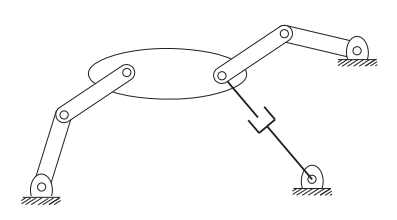
\includegraphics[width=\textwidth]{Images/image1.png}
                    \caption{Planar mechanism with \\ overlapping joints.}
                    \label{fig:mech_overlapping}
                \end{minipage}\hfill
                \begin{minipage}{0.5\textwidth}
                    The planar mechanism illustrated in fig: \ref{fig:mech_overlapping} has three links that meet at a single point on the right of the large link. Recalling that a joint by definition connects exactly two links, the joint at this point of intersection should not be regarded as a single revolute joint. Rather, it is correctly interpreted as two revolute joints overlapping each other. There is more than one way to derive the number of degrees of freedom of this mechanism using Gr\"{u}bler's formula: 
                \end{minipage} 
            \end{figure} 
            \begin{itemize}
                    \item i) The mechanism consists of eight links ($N = 8$), eight revolute joints and one prismatic joint ($J=9$). Substituting this into the formula yields: 
                    \begin{equation*} 
                        DoFs = 3(8-1-9)+9(1)=3
                    \end{equation*}
                    \item ii) Alternatively, the lower-right revolute–prismatic joint pair can be regarded as a single two-DoFs joint. In this case the number of links is $N = 7$, with seven revolute joints, and a single two-DoFs revolute–prismatic pair. Substituting into the formula:
                    \begin{equation*}
                        DoFs=3(7-1-8)+7(1)+1(2)=3
                    \end{equation*}
            \end{itemize}
        \item (Redundant constraints and singularities)
            \begin{figure}[htbp!]
                \centering
                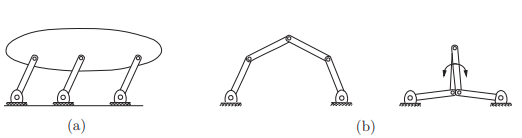
\includegraphics[width=0.5\linewidth]{Images/image3.png}
                \caption{(a) A parallelogram and (b) five-bar (in a regular and singular configuration) linkages}
                \label{fig:placeholder}
            \end{figure} \\
            For the parallelogram linkage, $N = 5, J = 6$, and $f_i = 1$ for each joint. From Gr\"{u}bler’s formula, the number of degrees of freedom is:
            \[3(5-1-6) + 6 = 0\]
            A mechanism with zero degrees of freedom is by definition a rigid structure. It is clear from examining the figure, though, that the mechanism can in fact move with one degree of freedom. Indeed, any one of the three parallel links, with its two joints, has no effect on the motion of the mechanism, so we should have calculated $DoFs = 3(4-1-4) + 4 = 1$. In other words, the constraints provided by the joints are not independent, as required by Gr\"{u}bler’s formula. \\
            A similar situation arises for the two-DoFs planar five-bar linkage: if the two joints connected to ground are locked at some fixed angle, the five-bar linkage should then become a rigid structure. However, if the two middle links are the same length and overlap each other, these overlapping links can rotate freely about the two overlapping joints.
            \newpage
        \item Delta Robot:
            \begin{figure}[htbp!]
                \begin{minipage}{0.4\textwidth}
                    \centering                  
                    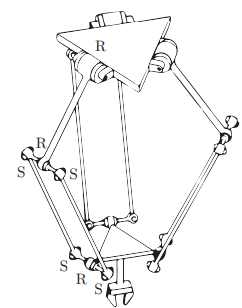
\includegraphics[width=\textwidth]{Images/image4.png}
                    \caption{Delta Robot}
                    \label{fig:delta_robot}
                \end{minipage}\hfill
                \begin{minipage}{0.5\textwidth}
                    The Delta robot consists of two platforms – the lower one mobile, the upper one stationary – connected by three legs. Each leg contains a parallelogram closed chain and consists of three revolute joints, four spherical joints, and five links. Adding the two platforms, there are $N = 17$ links and $J = 21$ joints (nine revolute and 12 spherical). By Gr\"{u}bler’s formula:
                    \[DoFs=6(17-1-21)+9(1)+12(3)=15\]
                    However, only three DoFs are actually visible from the end-effector perspective; this is one of the many perks of this robot, since it is capable of always maintaining its two platforms parallel to each other.
                \end{minipage} 
            \end{figure} 
        \end{itemize}
        Up until now we have only considered the dimension of the Configuration Space, i.e. the Degrees of Freedom; however, there is another aspect of great importance: the topology\footnote{In the context of pure mathematics, a \textit{topology} over a set $X$ is just a collection of sets, $\tau$, which are called \textit{open sets}, such that:
        \begin{itemize}
            \item $\emptyset,X\in \tau$ 
            \item If $O_i,O_j \in \tau$, then $O_i\cap O_j\in\tau$, for all $O_i,O_j \in \tau$.
            \item If $\mathcal{O}\subseteq \tau$, then $\cup_{O\in\mathcal{O}}O\in\tau$
        \end{itemize}
        Then, the couple $(X,\tau)$ is called a \textit{Topological Space}.}. \\
        Consider a plane and the surface of a sphere; to completely specify the position of a point in both spaces, there is need for only two coordinates (the $x,y$ coordinates in the plane or the longitude/latitude on the sphere), however the \textit{shape} of the two spaces is different: coordinates can wrap around on the surface of a sphere, meanwhile they cannot on the plane. Two spheres can be, however, be thought of as "the same" just deformed and are called \textit{topologically equivalent}; 
        \section{Topology Definition}
        A topological space can be expressed through different kind of definition. The main elements of topology are the open sets, the neighbourhoods and the points.
         More specifically, a topological space is a set whose elements are called points, along with an additional structure called a topology, which can be defined as a set of neighbourhoods for each point that satisfy some axioms formalizing the concept of closeness. There are several equivalent definitions of a topology, the most commonly used of which is the definition through open sets. 
         a topological space is, roughly speaking, a geometrical space in which closeness is defined but cannot necessarily be measured by a numeric distance.
        \begin{definition}
            \textit{Topological Equivalence}: A function $f:X \rightarrow Y$ between two topological spaces is a \textit{homeomorphism} if: 
            \begin{itemize}
                \item $f$ is a bijection.
                \item $f$ is continuous.
                \item $f^{-1}$ is continuous.
            \end{itemize}
            If such a function exists, then $X$ and $Y$ are \textit{topologically equivalent}. Geometrically, this means that one topological space can be continuously deformed into the other without cutting or adding any elements.
        \end{definition}
        As an example, the open set $(a,b)\subseteq \mathbb{R}$ is topologically equivalent to a line of real numbers by first folding it into a semicircle and then assigning its points to a line, as in the figure below.
        \begin{figure}[h!]
            \centering
            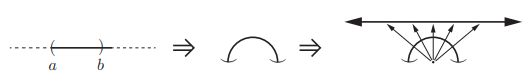
\includegraphics[width=0.5\linewidth]{Images/image5.png}
            \caption{: An open interval of the real line, denoted (a, b), can be deformed to an open semicircle. This open semicircle can then be deformed to the real line by the mapping illustrated: beginning from a point at the center of the semicircle, draw a ray that intersects the semicircle and then a line above the semicircle. These rays show that every point of the semicircle can be stretched to exactly one point on the line, and vice versa. Thus an open interval can be continuously deformed to a line, so an open interval and a line are topologically equivalent.
            }
            \label{fig:open_set_into_line}
        \end{figure}\\
        However, a closed set \textit{is not} topologically equivalent to a line, since it ends, the line does not. Note that the topology of a space is a fundamental property of the space itself and \textit{is independent} of how we choose coordinates to represent points in the space.
        Some C-spaces can be expressed as the Cartesian product of two or more spaces of lower dimension; that is, points in such a C-space can be represented as the union of the representations of points in the lower-dimensional spaces. For example:
        \begin{itemize}
            \item The C-space of a rigid body in the plane can be written as $\mathbb{R}\times S^1$, where $S^n$ is the surface of a $n$-dimensional space immersed into $(n+1)$-dimensional space.
            \item As we saw when we counted the degrees of freedom of a rigid body in three dimensions, the configuration of a rigid body can be described by a point in $\mathbb{R}^3$, plus a point on a two-dimensional sphere $S^2$, plus a point on a one-dimensional circle $S^1$, giving a total C-space of $\mathbb{R}^3 \times S^2 \times S^1$.
            \item The C-space of a PR robot arm can be written as $\mathbb{R}\times S^1$ (ignoring joints limits). 
        \end{itemize}
        While it is natural to choose a reference frame and length scale and to use a vector to represent points in a Euclidean space, representing a point on a curved space, such as a sphere, is less obvious. A choice of $n$ coordinates, or parameters, to represent an $n$-dimensional space is called an \textit{Explicit Parametrization} of the space. Such an explicit parametrization is only valid for a particular range of the parameters; there exists \textit{singularities} in parametric parametrizations. One such example is the North (or South) Pole of a sphere over which longitude-latitude coordinates are used; in these points, the coordinates wrap around their limiting values and the homeomorphism is undefined at the "wrapping" point (the inverse function is not defined). There are two ways to overcome the problem:
        \begin{itemize}
            \item Use more than one \textit{Coordinate Chart} on the space, where each coordinate chart is an explicit parametrization covering only a portion of the space such that, within each chart, there is no singularity. Then, one can simply switch between charts. If we define a set of singularity-free coordinate charts that overlap each other and cover the entire space they are said to form an \textit{Atlas}; the advantage here is:
            \begin{itemize}
                \item A minimum representation of space is maintained at all times.
            \end{itemize} 
            However the disadvantage is:
            \begin{itemize}
                \item A high amount of memory could be needed to remember each single chart.
            \end{itemize}
            \item Use an \textit{Implicit Representation}, which views the $n$-dimensional space as embedded in a Euclidean space of more than $n$ dimensions.  An implicit representation uses the coordinates of the higher-dimensional space but subjects these coordinates to constraints that reduce the number of degrees of freedom. The advantages here are:
            \begin{itemize}
                \item There are no singularities in the representation.
                \item Only one representation is needed to fully describe the space.
                \item It is way easier to find an implicit representation against an explicit one.
            \end{itemize}
            A disadvantage of this approach is that:
            \begin{itemize}
                \item The representation is constituted by a larger number of parameters than the system's number of DoFs.
            \end{itemize}
        \end{itemize}
        From now on, only implicit representations will be used.
\subsection{Exercises}
\paragraph{ProDrone a Six propellers plus two 5-DoFs arms drone:}
 \begin{figure}[htbp!]
                \begin{minipage}{0.4\textwidth}
                    \centering                  
                    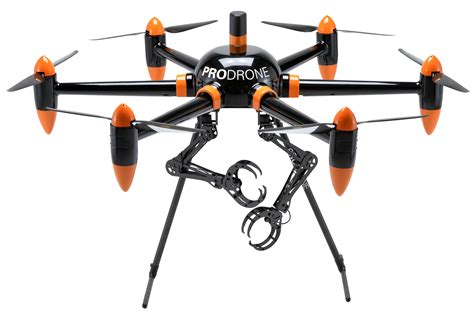
\includegraphics[width=\textwidth]{Images/ProDrone.jpg}
                    \caption{ProDrone}
                    \label{fig:ProDrone}
                    \end{minipage}
\hfill
                \begin{minipage}{0.6\textwidth}
        
\begin{itemize}
\item Body fixed on the ground
\begin{itemize}
\item 6 rotating propellers (1 link plus 1 rotational joint each)
\item 5 rotational joints for each arm
\item 1 Ground
\item DoFs = $6(6+5+5+1-1-6-5-5)+6+5+6 = 16$
\end{itemize}
\item Flying body
\begin{itemize}
\item 6 DoFs given by the spatial rigid body
\item DoFs = $16 + 6 = 22 $
\end{itemize}
\end{itemize}
                \end{minipage} 
            \end{figure}            
          
 \paragraph{Mobile Kuka a Mobile manipulator arms robot:}
 \begin{figure}[htbp!]
                \begin{minipage}{0.4\textwidth}
                    \centering                  
                    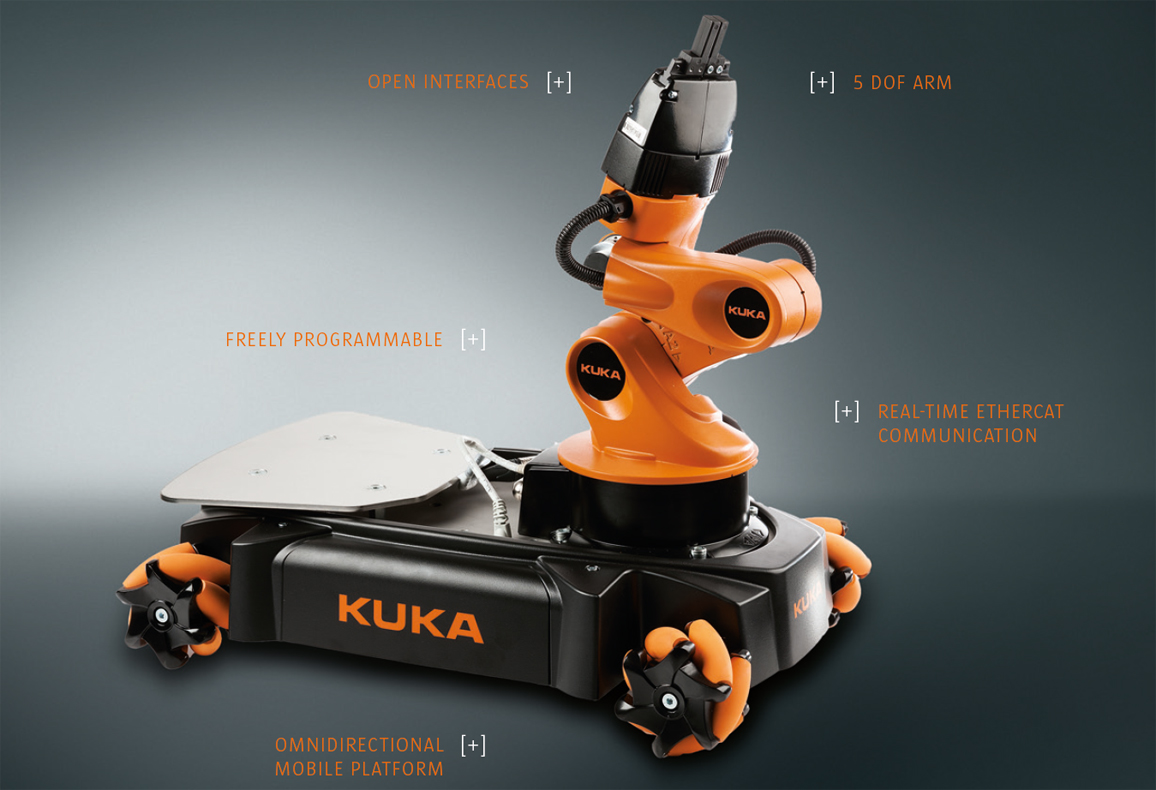
\includegraphics[width=\textwidth]{Images/Mobile_Kuka.jpg}
                    \caption{Mobile Kuka}
                    \label{fig:Mobile_Kuka}
                    \end{minipage}
\hfill
                \begin{minipage}{0.6\textwidth}
        
\begin{itemize}
\item KUKA youBot with 4 mecanum-wheels (omnidirecitonal base) plus 5-DoF robotic arm
\begin{itemize}
\item 4 wheels (1 link plus 1 rotational joint each)
\item A planar rigid body (3 DoFs)
\item 5 rotational joints for the arm
\item 12 DoFs
\end{itemize}
\end{itemize}
                \end{minipage} 
            \end{figure}
        \newpage
\section{Task space and Workspace}
        The C-space is related to the configuration of the entire robot; however, there are also other two spaces of interest, both only linked to the robot's end-effector: the \textit{Task Space} and the \textit{Workspace}. 
        \begin{definition}
            \textbf{Task Space}: The \textit{Task Space} is a space in which a robot's task can naturally be expressed.
        \end{definition}
        One example would be $\mathbb{R}^2$, a plane, for a robot whose task is to write on a sheet of paper; if the task is to manipulate a rigid body, a natural representation of the task space is the C-space of a rigid body, representing the position and orientation of a frame attached to the robot’s end-effector. This is the default representation of task space. Notice that the decision of how to define the task space \textit{is driven by the task, independently of the robot}. 
        \begin{definition}
            \textbf{Workspace}: The \textit{Workspace} is a specification of the configurations that the robot's end-effector can reach. The definition of the workspace is primarily driven by the robot’s structure, \textit{independently of the task}.
        \end{definition}
        The three spaces (Task, Work and C-space) are distinct but can overlap. A point in the task space or the workspace may be achievable by more than one robot configuration, meaning that the point is not a full specification of the robot’s configuration. For example, for an open-chain robot with seven joints, the six-DoF position and orientation of its end-effector does not fully specify the robot’s configuration. Some points in the task space may not be reachable at all by the robot, such as some points on a chalkboard. By definition, however, all points in the workspace are reachable by at least one configuration of the robot.
        \begin{figure}[htbp!]
                \begin{minipage}{0.5\textwidth}
                    \centering                  
                    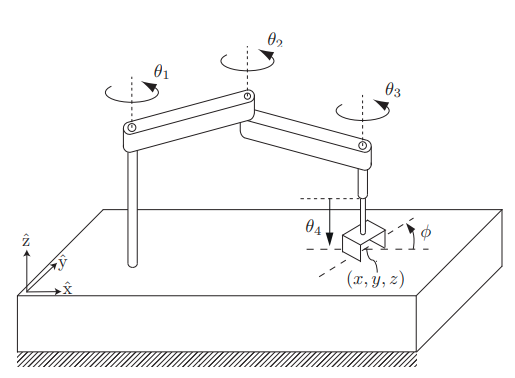
\includegraphics[width=\textwidth]{Images/image7.png}
                    \caption{SCARA Robot}
                    \label{fig:SCARA_robot}
                \end{minipage}% 
                \hfill%
                \begin{minipage}{0.5\textwidth}
                    To get an example, let's consider the SCARA robot in the picture. \\
                    The end-effector configuration is completely described by the four parameters $(x,y,z,\phi)$, where $\phi$ is the end-effector orientation in the $xy-$plane. Its task space would typically be defined as $\mathbb{R}^{3}\times S^1$, meanwhile its workspace would be typically defined as the reachable points in Cartesian space, regardless of orientation.
                \end{minipage} 
            \end{figure} 
            \section{Underactuation}
            As is known from physics, the motion of an arbitrary mechanical system occurs in such a way that the indefinite integral:
            \[A=\int_{t_i}^{t_f} \mathcal{L}(q,\dot{q})dt\]
            Called \textit{Action Integral}\footnote{There are many different definitions of \textit{action}, but this will suffice here.}, becomes stationary for all possible variations of the system's configurations, provided the initial and final state are given. The quantities $q, \dot{q}$ are called \textit{generalized coordinates} and \textit{generalized velocities} respectively, used to define the \textit{Lagrangian} $\mathcal{L}(q,\dot{q})=T-U$, where $T,U$ are the system's kinetic and potential energies. It is possible to use this definition to prove that the Action is stationary if and only if the \textit{Euler-Lagrange Equations} are satisfied: \footnote{This is \textit{Hamilton's Principle} or the \textit{Principle of Stationary Action}. A proof can be found in \cite{Taylor_ClassicalMechanics}.}
            \[\frac{d}{dt} \frac{\mathcal{\partial L}}{\partial\dot{q}}-\frac{\partial\mathcal{L}}{\partial q}=f\]
            Where $f$ is the vector of \textit{generalized forces} acting on the system. Notice that these are not necessarily forces in the classical sense of Newton's $F=ma$. \\
            The Euler-Lagrange Equations can be translated into matrix form, being completely equivalent to Newton's classic formulation of mechanics, such as:
            \[M(q)\ddot{q}+h(q,\dot{q})=f\]
            Where:
            \begin{itemize}
                \item $M(q) \in \mathbb{R}^{n \times n}$ is the \textit{Inertia Matrix}, which is positive definite and symmetric.
                \item $h(q,\dot{q})$ is the lumped vector of gravitational and non-inertial forces.
            \end{itemize}
            The relation can be inverted to extract the accelerations:
            \[\ddot{q}=-M^{-1}(q)h(q,\dot{q})+M^{-1}(q)f\]
            And if we define the generalized forces as functions of the inputs by defining the \textit{input matrix} $B$:
            \[f=B(q)\tau\]
            The system can be expressed in \textit{control-affine form}:
            \begin{equation}\label{control_affine_motion}
                \ddot{q}=b(q,\dot{q})+(M(q)^{-1}B(q))\tau=b(q,\dot{q})+G(q,\dot{q})\tau               
            \end{equation}
            Or in the general case:
            \[\ddot{q}=f(q,\dot{q},\tau,t)\]
            At this point, it should be natural to notice that it is not always the case that the control inputs can actually influence all the states, for instance in the case where the input matrix $B(q)$ is not full column-rank, meaning that the system has less inputs than states. In the general case this can be translated into a condition on the state-dynamics, in particular $f(\cdot)$ must be surjective. This is the problem of \textit{underactuation}:
            \begin{definition}
                \textbf{Underactuation}: a second order differential equation $\ddot{q}=f(q,\dot{q},\tau, t)$ is \textit{fully-actuated} in the state $x=(q,\dot{q})$ and the time $t$ if the map $f(\cdot)$ is surjective: 
                \[\forall \ddot{q}_{d}\in \mathbb{R}^{n} \exists u \in \mathbb{R}^{m}:\ddot{q}_d=f(q_0,\dot{q}_0,u,t)\]
                If this is not the case, the system is said to be \textit{underactuated}. A control-affine system is underactuated if:
                \[\text{Rank}_{\text{col}}(G(q,\dot{q}))<dim[q]\]
            \end{definition}
            It is important to notice that the system underactuation can change with either time, state or system constraints. However, usually a system is said to be underactuated if it so in every state and time. This also implies that most systems are underactuated, as for example is a quadcopter (being incapable of translating along the plane of the propellers at any time or initial state). \\
            Another keypoint about underactuation is that it depends on the mathematical model assumed for the system.  Imagine a two-link robot with two actuators. A typical model with rigid links could be fully actuated, but if we add extra DoFs to model small amounts of flexibility in the links then that system model could be underactuated. These two models describe the same robot, but at different levels of fidelity. Two actuators might be enough to completely control the joint angles, but not the joint angles and the flexing modes of the link. 
            \section{Controllability}
            Just as in linear system, in nonlinear systems it is also often useful to have a notion of \textit{controllability}.             
            \begin{definition}\label{controllability}
                \textbf{Controllability}: Let the system:
                \[\dot{x}=f(x,u)\]
                Be defined for $x \in D_{x,def}\subseteq \mathbb{R}^{n}$ and $u \in D_{u,ref} \subseteq \mathbb{R}^{m}$. Then, the system is said to be \textit{controllable} if any state $x_0 \in D_{x,def}$ can be transferred into any other $x_1 \in D_{x,ref}$ along a trajectory $x(t)\in D_{x,def}$ by an input function $u(t) \in D_{u}$ in a finite time interval $[0,T]$.
            \end{definition}
            Obviously, proving controllability for a general system is not an easy task. The notion of controllability can be specialized into other stricter notions, by defining a \textit{Reachable Set}:
            \begin{definition}
                \textbf{Reachable Set}: A \textit{Reachable Set} $R(x_0,T)$ is the set of points that may be reached starting from $x_0$ along any trajectory and any input in a finite time $T$.
            \end{definition}
            Notice that the definition implies that all trajectories linking $x_0$ with any element of $R(x_0,T)$ are completely contained into the set. The definition of Reachable Set gives the justification to define the concept of \textit{Small-Time Local Controllability}:
            \begin{definition}
                \textit{Small-Time Controllability}: Let a system:
                \[\dot{x}=f(x,u)\]
                be defined for $x \in D_{x,def} \subseteq \mathbb{R}^{n}$, $u \in D_{u,def} \subset \mathbb{R}^{m}$. Let $D_x \subseteq D_{x,ref}$ be an open set and $D_u \subseteq D_{u,def}$ a closed and bounded set. Then the system is called \textit{Small-Time Locally Controllable} if for every state $x_0\in D_x$, for $u(t) \in D_u$ where $0\leq t \leq T$, and for all $0 < T < \infty$ the sets $R(x_0,T)$ are neighborhoods \footnote{Topologically speaking, a set $N$ is a neighbor of $x$, if there exists an open set $O\in\tau$, where $\tau$ is the space topology, such that $x\in O$ and $O\subseteq N$. Basically, $x$ doesn't touch the "walls" or \textit{boundary} of $N$ and is safely inside of it.} of $x_0$.
            \end{definition}
            It is important to notice that, although every state inside $R(x_0,T)$ can be reached, this doesn't necessarily imply that the system can evolve along all possible trajectories inside $R(x_0,T)$. The following theorem is also useful:
            \begin{theorem}
                A system that is small-time locally controllable on a path-connected set $D_x$ is controllable on this set.
            \end{theorem}
            Finally, the notion of \textit{Omnidirectional Controllability} is introduced:
            \begin{definition}\label{Omnidirectional_Controllability}
                \textit{Omnidirectional Controllability}: Let a system:
                \begin{equation*}
                    \dot{x}=f(x,u)
                \end{equation*}
                be defined for $x\in D_{x,def}\subseteq \mathbb{R}^{n}$, $u \in D_{u,def} \subseteq \mathbb{R}^{m}$. Let $D_x \subseteq D_{x,def}$ be a path-connected set and $D_u \subseteq D_{u,def}$. Then the system is called \textit{Omnidirectionally Controllable} if any state $x_0 \in D_x$ can be transferred to any other $x_e \in D_x$ by an input function $u(t) \in D_u$ along \textit{any arbitrary} trajectory $x(t) \in D_x$ within a finite time interval $[0,T]$.
            \end{definition}
            \begin{figure}[htbp!]
                \begin{minipage}{0.3\textwidth}
                    \centering
                    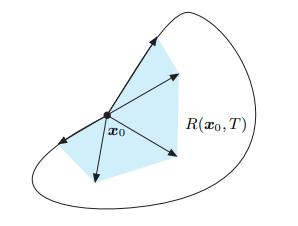
\includegraphics[width=\textwidth]{Images/image9.png}
                    \caption{Controllability: 
                     $R(x_0,T )$ is not a neighborhood of $x_0$.}
                    \label{fig:controllability}
                \end{minipage}
                \hfill               
                \begin{minipage}{0.3\textwidth}
                    \centering
                    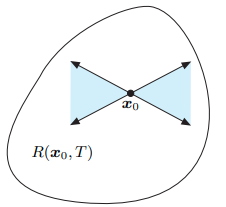
\includegraphics[width=0.5\linewidth]{Images/image10.png}
                    \caption{Small-Time Local Controllability: \\
                    In general, trajectories cannot progress from the point $x_0$ in all directions.}
                    \label{fig:small_time_controllability}
                \end{minipage}
                \hfill
                \begin{minipage}{0.3\textwidth}
                    \centering
                    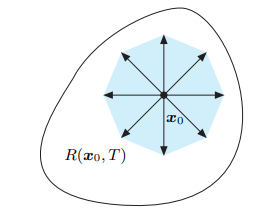
\includegraphics[width=0.5\linewidth]{Images/image11.png}
                    \caption{Omnidirectional Controllability: \\
                    The trajectories can progress starting from $x_0$ in all directions.}
                    \label{fig:omni_controllability}
                \end{minipage} \hfill
            \end{figure}
            The concept of controllability can be more easily applied to control-affine systems, by defining the \textit{Accessibility Distribution}:
            \begin{definition}
                \textbf{Accessibility Distribution}: Let:
                \begin{equation*}
                    \dot{x}=f(x)+\sum_{i=0}^{d}g_{i}(x)u_i
                \end{equation*}
                Be a control-affine system. Then, let the \textit{Accessibility Distribution} $\Delta_{A}$ be the distribution generated by the vector fields $f,g_i$ and all the Lie Brackets that can be generated by them. 
            \end{definition}
            Assuming that the vector fields are all $C^\infty$ \footnote{Meaning that they are continuously differentiable, for every order of derivation: $\frac{d^{(n)}}{dx^{(n)}}f$ is continuously differentiable, for all $n \in \mathbb{N}$.}, then if $\dim(\Delta_a)=n$ for all times, the accessible set $R(x_0,T)$ has a non-empty interior: the system is always accessible. This is summarized by the theorem:
            \begin{theorem}\label{Accessibility_rank_condition}
                \textbf{Accessibility Rank Condition}: A Control-Affine system:
                \begin{equation*}
                    \dot{x} = f(x)+\sum_{i=1}^{d}g_i(x)u_i
                \end{equation*}
                Where $f,g_i$, for $i \in \{1,\dots,d\}$ are $C^\infty$, is accessible from $x_0$ if the following \textit{accessibility rank condition} is satisfied:
                \begin{equation}\label{acc_rank_cond}
                    \dim(\Delta_a(x_0))=n
                \end{equation}
                If the condition is satisfied for all $x \in U \subseteq\mathbb{R}^{n}$, then the system is controllable on $U$.
            \end{theorem}
            Geometrically speaking, this statement implies that the system can move along any direction on the tangent hyperplane to the system's dynamics manifold at the point $x\in U$.